\documentclass[sigplan,11pt,nonacm]{acmart}
\settopmatter{printfolios}

\usepackage{booktabs} % For formal tables
\usepackage{subcaption}
\usepackage{tikz}
\usetikzlibrary{fit}
\usepackage{pgfplots}
\usepackage{pgfplotstable}
\usepackage{hyphenat}
\usepackage{todonotes}
\usepackage[babel]{csquotes}
\usepackage{listings}
\usepackage{listings-rust}
\usepackage{microtype}

\definecolor{cgreen}{RGB}{60,201,65}
\definecolor{dkgreen}{rgb}{0,0.6,0}
\definecolor{mauve}{rgb}{0.58,0,0.82}

\lstset{frame=tb,
  % aboveskip=3mm,
  % belowskip=3mm,
  showstringspaces=false,
  columns=flexible,
  basicstyle={\small\ttfamily},
  numbers=left,
  numbersep=5pt,
  xleftmargin=\parindent,
  numberstyle=\color{gray},
  keywordstyle=\bfseries\color{blue},
  commentstyle=\color{dkgreen},
  stringstyle=\color{mauve},
  breaklines=true,
  % breakatwhitespace=true,
  tabsize=2
}
\pagenumbering{gobble}


\begin{document}
\title{Ownership types in theory and practice (in Rust)}
\author{Fritz Rehde}
\affiliation{%
  \institution{Technical University of Munich}
  \country{Germany}
}
\email{fritz.rehde@tum.de}


% TODO: brief overview of sections somewhere (maybe end of introduction)

\begin{abstract}
% Abstract: Brief summary of area, problem, approach, key result

Object aliasing is the concept of accessing the same memory through different symbolic names in object-oriented programming languages.
Many programming bugs are created through unintentional aliases, which are hard to detect and can lead to unexpected side effects.
Ownership types are one solution that attempts to prevent many alias-related bugs.
The premise of ownership types is that not only the fields of an object are protected from external access, but also all objects stored in those fields.
This is done by allowing objects to take ownership of other objects.

This paper depicts some of the different kinds of ownership types, explains how the modern programming language Rust uses ownership types and evaluates Rust's implementation by comparing its use of the ownership concept to that of another popular systems programming language, namely C++.

\end{abstract}


\keywords{Ownership, Type, Safety, Rust}
\maketitle


\section{Introduction}
\label{sec:introduction}
% Introduction: introduce area, problem, approach, key results, contributions, outline

One of the main goals of ownership types is to improve memory safety.
Understanding memory-related bugs will, therefore, help in understanding why ownership types are useful.


\subsection{Memory Safety}
\label{sec:memory-safety}

Memory safety refers to the state of a program where memory pointers or references always refer to valid memory.

The tech giants Google \cite{google-memory-safety} and Microsoft \cite{microsoft-memory-safety} have both revealed that around 70 percent of their vulnerabilities were the result of memory safety issues.
The importance of memory safety is further underlined by the fact that the National Security Agency of the United States of America has published a Cybersecurity Information Sheet \cite{nsa-memory-safety} on the topic, the contents of which are described in the following section.

There are a variety of potential occurrences of memory management issues.
Examples include \emph{buffer overflows}, where data is accessed outside the bounds of an array, \emph{memory leaks}, where the programmer forgets to free memory that has been allocated, causing the program to, eventually, run out of memory, \emph{Use-After-Free}, where memory is accessed after it has been freed, \emph{Double-Free}, where memory is freed again after it had already been freed before, and the use of uninitialized memory.
These issues can not only enable potential malicious exploits, but they can also result in incorrect program results, the decrease of a program's performance or seemingly random program crashes.

Commonly used programming languages, such as C and C++, provide a lot of freedom and flexibility in memory management, but this comes at the cost of heavily relying on the programmer to perform the needed checks on memory references.
Furthermore, the programmer must perform rigorous testing to ensure that the software handles surprising conditions.
Even though software analysis tools can detect many instances of memory management issues, the NSA recommends the use of inherently memory-safe languages.


\paragraph{Example}

Ralf Jung \cite{understanding-evolving-rust} provides the following common example of how ownership types can prevent a memory safety issue.

First, we will explore how a memory safety problem is created in the following C++ code snippet that does not use the ownership concept.

\begin{lstlisting}[language=C++,captionpos=b,caption={C++ use-after-free \cite{understanding-evolving-rust}}]
std::vector<int> v { 10, 11 };
int *vptr = &v[1]; // points into v
v.push_back(12);
std::cout << *vptr; // bug (use-after-free)
\end{lstlisting}

We initialize a vector \emph{v} that contains two integers stored in a buffer in memory.
Next, we create a pointer \emph{vptr} that points into this buffer, specifically to the place where the second element (with current value 11) is stored.
Now, both \emph{v} and \emph{vptr} point to (overlapping parts of) the same buffer.
We say that the two pointers are aliasing.
Then, we push a new element to the end of \emph{v}.
If the vector's capacity were large enough, the new element would be appended to the buffer.
However, we will assume there is no more space for an additional element, so a new buffer is allocated, and all the existing elements are moved over.
This case is interesting because \emph{vptr} still points to the old buffer!
In other words, adding a new element to \emph{v} has turned \emph{vptr} into a dangling pointer.
Therefore, trying to access the value, which the dangling pointer \emph{vptr} points to, will cause a use-after-free bug.
More generally, we can observe that an action through a pointer (\emph{v}) will also affect all of its aliases (\emph{vptr}), even though these aliases might not expect a change.
The main problem here is that such memory issues cannot be detected at compile time.

Now, we will demonstrate how ownership types in Rust allow the compiler to detect such a use-after-free bug.
Consider the following Rust translation of our C++ example:

\begin{lstlisting}[language=Rust,captionpos=b,caption={Rust use-after-free \cite{understanding-evolving-rust}}]
let mut v = vec![10, 11];
let vptr = &mut v[1]; // points into v
v.push(12);
println!("{}", *vptr); // compiler error
\end{lstlisting}

Syntactically, the C++ and Rust versions are very similar.
Notably, the \emph{push} method in line 3 has the following signature: \verb|pub fn push(&mut self, value: T)| \cite{rust-vector-documentation}.
While the C++ version will compile successfully, causing a run-time security vulnerability, the Rust compiler shows an error: "Cannot borrow \emph{v} as mutable more than once at a time."
For now, it suffices to say that the Rust compiler disallows both lines 2 and 3 to create mutable references to \emph{v} if one of the mutable references is used later (like \emph{vptr} is in line 4).
In \ref{sec:rust-references} and \ref{sec:rust-lifetimes}, we will explain in more detail how the Rust borrow-checker is able to detect this problem using Rust's ownership rules.


\subsection{State of the art}
\label{sec:state-of-the-art}

The concept of ownership types provides one of the solutions aiming to eliminate many of the described memory-related bugs.
Potential solutions to the aliasing problem include banning aliases altogether, clearly advertising aliases or managing and controlling their effects \cite{ownership-types-survey}.
Many different flavors of ownership types have been explored.
In this paper, state-of-the-art implementations of the ownership types concept, such as owners-as-dominators and owners-as-modifiers, will be explored further.
These approaches differ in what kind of, if any, aliases they allow.


% Main part (approach, evaluation, discussion, etc.)

\section{Ownership types in theory}
\label{sec:theory}

In object-oriented programs, an object can reference any other object and read and modify its fields through direct field accesses or method calls.
Such programs with arbitrary object structures are difficult to understand, maintain, and reason about. \cite{lightweight-ownership}

Ownership types can limit which objects can be referenced, and can specify whether the referenced objects may be mutated or just read from.

If not otherwise indicated, all of the information gathered in this chapter stems from the Ownership Types Survey \cite{ownership-types-survey}.


\subsection{Domain specific terms}
\label{sec:domain-specific-terms}

In the following, some terms from the Ownership Types survey \cite{ownership-types-survey}, which are commonly used in this chapter, are defined.

The core concept of ownership types is that each object is \emph{owned} by (at most) one other object, called its \emph{owner}.
Objects are organized into different \emph{ownership contexts}.
An ownership context is the set of all objects with the same owner.
Objects that are in the same ownership context, meaning they share the same owner, are called \emph{siblings} or \emph{peers}.
More informally, an object's ownership context can also be visualized as a box into which all of its owned objects are placed, to store and protect these objects.
Each object is considered to be \emph{inside} the object whose ownership context box it is placed in.
There also exists a more formal definition of the \emph{inside} relation:
Given the two objects \emph{a} and \emph{b}, \emph{a} is \emph{inside} \emph{b} if \emph{a} is the same object as \emph{b} or \emph{a} is \emph{owned} by \emph{b}, transitively.
The \emph{outside} relation is the converse of the \emph{inside} relation.
This hierarchy induces a nesting relationship between objects. \cite{ownership-types-survey}


\subsection{Owners-as-dominators}
\label{sec:owners-as-dominators}

One flavor of ownership types is the \emph{owners-as-dominators} model \cite{ownership-types-survey}, which is an implementation of the core encapsulation mechanism from the original Flexible Alias Protection concept \cite{flexible-alias-protection}.

Zhao and Boyland \cite{permission-ownership-types} specify that, with owners-as-dominators, each regular object is owned by exactly one object and can be the owner of zero or more objects.
Objects can also be owned by a special global object called \emph{world}, which cannot be owned anymore.
This \emph{world} object is the root of the acyclic ownership hierarchy tree that represents the ownership relation.
In this tree structure, each object is inside its owner.
This model is named \emph{owners-as-dominators} because any object acting as an owner is considered to be a \emph{dominator} for all of its owned objects.

The ownership survey \cite{ownership-types-survey} defines that at least one of the following rules must apply for object \emph{a} to validly reference \emph{b}.
\begin{enumerate}
  \item \emph{a} is the owner of \emph{b},
  \item \emph{a} and \emph{b} are siblings, or
  \item \emph{b} is outside of \emph{a}.
\end{enumerate}

\begin{figure}
  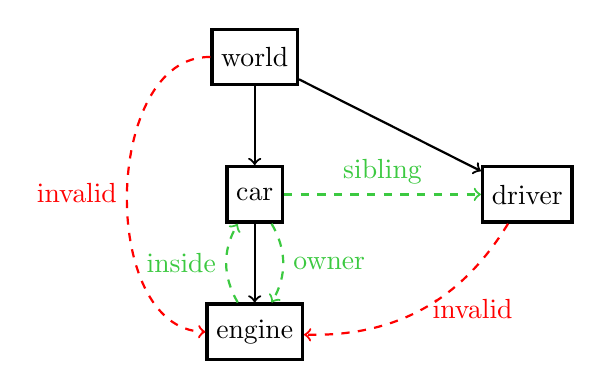
\begin{tikzpicture}[object/.style={rectangle, draw, very thick, minimum size=20}]
    \node[object] (World) {world};
    \node[object] (Car) [below=of World] {car};
    \node[object] (Driver) [right=of Car,xshift=1.5cm] {driver};
    \node[object] (Engine) [below=of Car] {engine};

    \draw[->,thick] (World) to (Car);
    \draw[->,thick] (World) to (Driver);
    \draw[->,thick] (Car) to (Engine);

    \draw[->,thick,dashed,cgreen] (Car) edge[bend left] node[right] {owner} (Engine);
    \draw[->,thick,dashed,cgreen] (Engine) edge[bend left] node[left] {inside} (Car);
    \draw[->,thick,dashed,cgreen] (Car) edge node[above] {sibling} (Driver);
    \draw[->,thick,dashed,red] (World) edge[bend right=90] node[left] {invalid} (Engine);
    \draw[->,thick,dashed,red] (Driver) edge[bend left] node[right] {invalid} (Engine);
  \end{tikzpicture}

  \caption{Owners-as-dominators \cite{flexible-alias-protection}: Solid lines indicate "owns", dotted lines indicate "references".}
  \label{fig:owners-as-dominators}
\end{figure}

Figure \ref{fig:owners-as-dominators} was adapted from an example by Clarke et al. \cite{flexible-alias-protection} and demonstrates valid (green) and invalid (red) references in an ownership hierarchy.
Each of the three reference-validity rules that were defined previously will be illustrated using this example figure.


\paragraph{Owner}

The object \emph{car} owns the object \emph{engine}, meaning that \emph{car} can validly reference \emph{engine} according to the first rule.

An owner being able to access its owned objects is the most trivial and intuitive rule.


\paragraph{Sibling}

The objects \emph{car} and \emph{driver} are siblings because they are both in the ownership context of the object \emph{world}.
This means that they can validly reference each other according to the second rule.

The lack of further rules implies that siblings are the only objects that an object can validly reference besides the objects it owns and the objects it is inside of.
The sibling relationship would, therefore, be used for objects that exist independently but should still be able to interact with each other.


\paragraph{Outside/inside}

The object \emph{engine} is inside the object \emph{car} because \emph{engine} is owned by \emph{car}.
Conversely, \emph{car} is outside \emph{engine}.
Therefore, according to the third rule, \emph{engine} can validly reference \emph{car}.

The original Flexible Alias Protection model, on which these ownership types are based, imposed the same restriction.
"The only objects that can access [an object] are the object that owns it, and other objects inside that [object]" \cite{flexible-alias-protection}.
The implication is that this model only protects objects from external access.
However, internally, an object can still access its owner (and its owner's owner etc.).

Dietl and Müller \cite{lightweight-ownership} point out that there exist several slightly different specifications of the owners-as-dominators model.
They claim that Clarke's owners-as-dominators property \cite{ownership-types-survey} is weaker than others "by allowing instances of inner classes to access the representation of the instance of the outer class they are associated with" \cite{lightweight-ownership}, which we have already identified in the third rule.
They state that, thereby, this owners-as-dominators model can handle iterators, but not more general forms of sharing \cite{lightweight-ownership}.


\paragraph{Further implications}

Primarily, these three rules imply that any external reference to an object is only possible through its owner.
This is exemplified in Figure \ref{fig:owners-as-dominators} where the object \emph{world} is trying to access the object \emph{engine}, which is not allowed because \emph{world} is neither a direct owner of, a sibling of or inside of \emph{engine}.
Instead, \emph{world} could only reference \emph{engine} through the \emph{engine}'s owner \emph{car}.

According to Dietl and Müller \cite{lightweight-ownership}, the owners-as-dominators model restricts \emph{where} references are allowed to point to.
Any object that can be validly referenced may be mutated through that reference.

Its strictness can be seen as both an advantage and a disadvantage of the owners-as-dominators model.
The advantage is that the model provides a simple, clear and strong guarantee that allows for reasoning about various properties of the code.
However, it also makes programming more difficult by not allowing common idioms that involve aliasing. \cite{ownership-types-survey}


\subsection{Owners-as-modifiers}
\label{sec:owners-as-modifiers}

Another kind is the \emph{owners-as-modifiers} model \cite{ownership-types-survey}, which is a weaker form of owners-as-dominators that additionally allows read-only references.
A read-only reference can only be used to read fields and call \emph{pure methods}.
Pure methods are defined as methods that do not modify the fields of any existing objects. \cite{ownership-types-survey}

For \emph{a} to validly reference \emph{b} through reference \emph{r}, at least one of the following rules \cite{ownership-types-survey} must apply.
\begin{enumerate}
  \item \emph{a} is the owner of \emph{b},
  \item \emph{a} and \emph{b} are siblings, or
  \item \emph{b} is outside of \emph{a}, or
  \item \emph{r} is a read-only reference and only pure methods can be called on it.
\end{enumerate}
We can see that the owners-as-modifiers rules extend the rules specified for owners-as-dominators.
The only additional rule is that a reference can also be valid if it is a read-only reference and only pure methods are being called on it.

\begin{figure}
  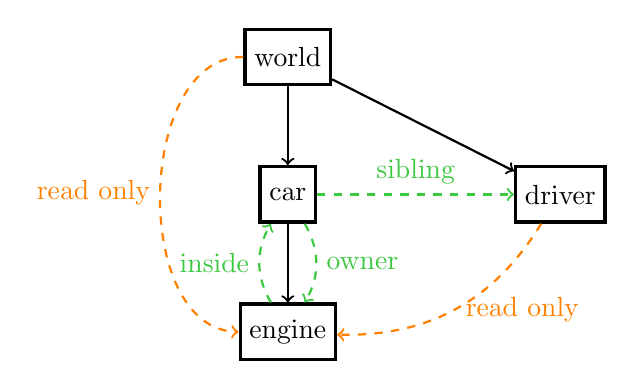
\begin{tikzpicture}[object/.style={rectangle, draw, very thick, minimum size=20}]
    \node[object] (World) {world};
    \node[object] (Car) [below=of World] {car};
    \node[object] (Driver) [right=of Car,xshift=1.5cm] {driver};
    \node[object] (Engine) [below=of Car] {engine};

    \draw[->,thick] (World) to (Car);
    \draw[->,thick] (World) to (Driver);
    \draw[->,thick] (Car) to (Engine);

    \draw[->,thick,dashed,cgreen] (Car) edge[bend left] node[right] {owner} (Engine);
    \draw[->,thick,dashed,cgreen] (Engine) edge[bend left] node[left] {inside} (Car);
    \draw[->,thick,dashed,cgreen] (Car) edge node[above] {sibling} (Driver);
    \draw[->,thick,dashed,orange] (World) edge[bend right=90] node[left] {read only} (Engine);
    \draw[->,thick,dashed,orange] (Driver) edge[bend left] node[right] {read only} (Engine);
  \end{tikzpicture}

  \caption{Owners-as-modifiers \cite{ownership-types-survey}: Solid lines indicate "owns", dotted lines indicate "references".}
  \label{fig:owners-as-modifiers}
\end{figure}

\paragraph{Implications}

Dietl and Müller \cite{lightweight-ownership} suggest that the owners-as-modifiers approach allows references to point to objects in arbitrary contexts, but restricts \emph{how} references can be used.
In particular, any object can be referenced by any given object.
However, only an object that is the owner of, a sibling of or inside of another given object may receive a reference to that object that allows mutating the object.
Figure \ref{fig:owners-as-modifiers} demonstrates that all other objects, such as \emph{world} or \emph{driver}, which may not be allowed to obtain a mutable reference to an object for the reasons above, can still receive read access to said object.

The advantage of this model is that it expands the programming possibilities of the owners-as-dominators principle and fulfills the requirements needed for the verification of the functional correctness of object-oriented programs. \cite{ownership-types-survey}
% TODO: which requirements for verficiation?


\section{Implementation in Rust}
\label{sec:implementation-in-rust}

Rust's notion of ownership is the culmination of a long line of work.
Many researchers have aimed to develop systems for functional programming without garbage collection.
According to Weiss et al. \cite{oxide}, it is best understood that Rust's ownership model is based on Baker's work on Linear Lisp \cite{linear-lisp} where linearity enabled efficient reuse of objects in memory without garbage collection.
Furthermore, the resemblance is especially strong between Rust \emph{without} borrowing (the Rust terminology for referencing, explained in \ref{sec:rust-references}) and Baker's 'use-once' variables.
'Use-once' variables are bound to linear (unshared, unaliased or singly-referenced) objects and are cheap to access and manage because they require no synchronization or tracing garbage collection \cite{use-once}.

However, techniques like the 'use-once' variables differentiate themselves from Rust by requiring that all objects must be managed uniquely.
Instead, Rust allows the use of shared references without mutation or unique references with unguarded mutation \cite{oxide}.

One can argue that Rust's ownership system is an extended version of the ownership model \emph{owners-as-modifiers}.
The owners-as-modifiers and Rust approaches differentiate themselves from the owners-as-dominators model, since they both allow read-only references to any object.
Furthermore, as will be discussed in \ref{sec:rust-references}, Rust allows both read-only and mutable references in a controlled manner.
This allows for expressing more programming idioms.

Most of the Rust-related information gathered in this chapter is derived from the "Understanding Ownership" section in the Rust Book \cite{rust-book}.


\subsection{Memory allocation system}
\label{sec:memory-allocation}

We will begin our exploration of ownership types in Rust by defining its memory allocation system.
There are two major requirements that a memory allocation system must fulfill:
At runtime, memory can be requested from the memory allocator, and there exists a mechanism for memory to be freed by the memory allocator.

The first requirement is trivial.

One possible implementation of the second requirement is using a garbage collector, which keeps track of and cleans up memory that is no longer used.
This, however, has a runtime performance overhead and can lead to a non-deterministic cleanup of resources. \cite{understanding-evolving-rust}

Another more traditional solution is requiring memory to be freed explicitly.
This is a notorious source of bugs.
If memory is never freed because it was forgotten, memory is wasted.
If it is freed multiple times or accessed again after having been freed, it will result in undefined behavior.

The ideal solution pairs one \emph{allocate} with exactly one \emph{free}.
Rust uses neither a garbage collector nor requires memory to be freed manually.
Instead, the concept of ownership is leveraged to determine when to free memory.

The Rust Book \cite{rust-book} defines ownership as a set of rules that govern how it manages memory.
The compiler checks whether these rules are adhered to and does not compile the program if they are violated.
The ownership rules in Rust are as follows:
\begin{enumerate}
  \item Each value in Rust has an owner.
  \item There can only be one owner at a time.
  \item When the owner goes out of scope, the value will be \emph{dropped}.
\end{enumerate}
The scope of a value is the range within a program in which it is valid.
Rust automatically calls the function \emph{drop} when a value goes out of scope, which frees the associated memory.

The following describes how the concept of ownership is implemented in Rust.


\subsection{Transferring ownership}
\label{sec:rust-transferring-ownership}

One common restriction to the early ownership systems is that the owner of an object must be set upon creation and then fixed for the lifetime of the object \cite{ownership-types-survey}.
Rust extends these original ownership concepts by allowing the ownership of an object to be transferred.

First, one must differentiate between values that are stored on the stack and those stored on the heap.
In Rust, primitive data types (e.g. signed 32-bit integers \emph{i32}) are stored on the stack since their sizes are small and known at compile time.
In contrast, values are stored on the heap if their size is dynamic and, therefore, unknown at compile time.

\paragraph{Heap-based values}

In addition to the memory safety that ownership types provide, ownership transfers can also reduce redundant copy operations.
Since heap-based values could be arbitrarily large at runtime, copying the whole value instead of transferring ownership could be very inefficient.
There are several different scenarios in which ownership is transferred.

In the simplest scenario, ownership is transferred from the variable \emph{a} to the variable \emph{b} when the variable \emph{b} is assigned to the value of \emph{a}.
\footnote{For the sake of simplicity, the main function is omitted in some code snippets}

\begin{lstlisting}[language=Rust,captionpos=b,caption={Rust simple heap-based move}]
let a = HeapBasedType::default();
let b = a;
\end{lstlisting}
In Rust terminology, \emph{a} is \emph{moved} into \emph{b}.
After the move, \emph{a} is no longer valid, and \emph{b} is the new owner of the value.

Heap-based values will always be generated by a function at runtime.
In the above example, the return value of the function \verb|HeapBasedType::default()| is moved into \emph{a}.
Furthermore, one can generalize the above scenario to ownership being transferred from the variable \emph{a} to the variable \emph{b} when \emph{b} is assigned to the return value \emph{a} of \emph{foo}.
\begin{lstlisting}[language=Rust,captionpos=b,caption={Rust heap-based move out of function}]
fn main() {
  let b = foo();
}
fn foo() {
  let a = HeapBasedType::default();
  a
}
\end{lstlisting}

Lastly, ownership is transferred from the variable \emph{a} to the variable \emph{b} when \emph{a} is passed to function \emph{foo}, which takes a parameter \emph{b}.
\begin{lstlisting}[language=Rust,captionpos=b,caption={Rust heap-based move into function}]
fn main() {
  let a = HeapBasedType::default();
  foo(a);
}
fn foo(b: HeapBasedType) {
  // do something with b
}
\end{lstlisting}
In \emph{foo}, \emph{b} is the owner of the value until it is \emph{dropped} at the end of the function.
Again, accessing the moved-from variable after the ownership of that value has been transferred elsewhere will lead to a compile-time error.
In this case, trying to access \emph{a} after line 3 would not compile, as \emph{a} is no longer the owner of the value.

The heap-allocated \emph{String} type in Rust provides a good example of heap-based ownership transfer.
\begin{lstlisting}[language=Rust,captionpos=b,caption={Rust String move}]
let x: String = String::from("hello world");
let y: String = x;
println!("x: {}, y: {}", x, y); // error
\end{lstlisting}
After \emph{x} is moved into \emph{y} in line 2, \emph{x} is no longer valid.
Therefore, Rust does not allow accessing the moved-from variable \emph{x} in the third line, and the program will not compile.


\paragraph{Stack-based values}

In contrast to heap-based values, the size of stack-based values is known at compile time and is usually small.
Therefore, stack-based values in Rust are \emph{copied} instead of \emph{moved}.
Internally, this works because primitive types are annotated with the \emph{Copy} trait.

The following piece of code \cite{rust-book}, which is similar to the code from above but replaces the \emph{String} type with primitive integers, demonstrates how stack-based values are \emph{copied} instead of \emph{moved} into other variables in Rust.
\begin{lstlisting}[language=Rust,captionpos=b,caption={Rust stack-based move}]
let x: i32 = 42;
let y: i32 = x;
println!("x: {}, y: {}", x, y);
\end{lstlisting}
The value of \emph{x} is copied into \emph{y}, after which both variables are still valid.
Therefore, the program compiles and "x: 42, y: 42" is printed to stdout.


\paragraph{Moving fields out of structs}

In their work on the owners-as-modifiers property, Clarke et al. \cite{ownership-types-survey} emphasize that rather than simply protecting the fields of an object from external access, ownership types also protect the objects stored in the fields, thereby enabling an object to claim (exclusive) ownership of and access to other objects.
This notion has been implemented in the Rust ownership system as well.
The following example illustrates that not only whole objects, but also the fields of structures, can be moved into other objects.

\begin{lstlisting}[language=Rust,captionpos=b,caption={Rust moving struct fields}]
struct Car {
  engine: Engine,
  wheels: Wheels,
}
fn main() {
  let car = Car::default();
  let moved_engine = car.engine; // move
  car.drive() // error: use of partially moved value: 'car'
}
\end{lstlisting}

In line 7, we perform a so-called \emph{partial move}, which means that parts of the variable \emph{car} are moved into \emph{engine}.
The untouched parts, such as \emph{wheels} in our example, will still be accessible afterward.
After we move the \emph{engine} field out of the \emph{car} structure, however, the parent variable \emph{car} cannot be used as a whole again.
Therefore, the compiler will complain that we want to call the \emph{drive} method on the partially moved value \emph{car}.


\subsection{The Clone trait}
\label{sec:rust-clone-trait}

By default and by design, Rust will never automatically create deep copies of data stored on the heap.
To do so, one must explicitly call the \emph{clone} method on an object.

The following adjustment to the code snippet from above creates a deep copy of \emph{x} and compiles successfully.
\begin{lstlisting}[language=Rust,captionpos=b,caption={Rust copy with clone}]
let x: String = String::from("hello world");
let y: String = x.clone();
println!("x: {}, y: {}", x, y);
\end{lstlisting}


\subsection{Immutability}
\label{sec:rust-immutability}

By default, all values in Rust are immutable.
An object is defined as immutable if its state cannot be modified after its creation.
In Rust, mutable values and references must be explicitly created using the \emph{mut} keyword.

For example, an integer can only be reassigned if it is mutable.
\begin{lstlisting}[language=Rust,captionpos=b,caption={Rust mutable variables}]
let a = 42;
a = 24; // compile error
let mut b = 42;
b = 24; // valid
\end{lstlisting}


\subsection{References and borrowing}
\label{sec:rust-references}

Object aliasing has already been defined as the concept of accessing the same memory through different symbolic names.
Specifically, the \emph{owners-as-modifiers} approach relies on implementing the aliasing concept.
Therefore, any programming language based on this form of ownership type must provide a way of achieving this behavior.
One way of implementing this behavior is through \emph{pointers}, which are commonly used in low-level programming languages.
However, even though they exist, "working with raw pointers in Rust is uncommon [and] typically limited to a few patterns" \cite{rust-pointer-documentation}.
Instead, Rust uses \emph{references} as the preferred way of implementing aliasing.

In Rust, a \emph{reference} is an address that points to a value that is owned by another variable.
Unlike traditional \emph{pointers}, a reference is guaranteed by the compiler to point to a valid value.
In Rust terminology, creating a reference is called \emph{borrowing}.
A reference does not own the value it points to.
Therefore, only the reference itself, not the value that the reference has borrowed, is dropped at the end of the reference's scope.
Borrowing is useful for performing an operation on a value without taking ownership of it.
Rust supports creating immutable and mutable references.

\paragraph{Lifetimes}
\label{sec:rust-lifetimes}

One detail we must discuss before providing details on immutable and mutable references is that every reference in Rust has a \emph{lifetime} \cite{rust-book}.
References borrow ownership and thus grant temporary access to a data structure \cite{understanding-evolving-rust}.
A lifetime is a construct that the compiler, or more specifically, its \emph{borrow checker}, uses to ensure that all borrows are valid \cite{rust-by-example}.
The full form of a reference type, including lifetime annotations, is \verb|&'a mut T| or \verb|&'a T|, where \verb|'a| is the lifetime of the reference.
Our examples have not included explicit lifetime annotations until now because the compiler uses some conventions to elide them.
To ensure references get used correctly, the compiler enforces the following two constraints \cite{understanding-evolving-rust}:
\begin{enumerate}
  \item The reference can only be used while its lifetime is ongoing, and
  \item the original referent is not used at all (for mutable references) or does not get mutated (for immutable references) until the lifetime of the newly created reference has expired.
\end{enumerate}
The lifetime of a reference starts where it is introduced and extends until the last time it is used.

First, we will provide an example of a program that requires explicit lifetime annotations.

\begin{lstlisting}[language=Rust,captionpos=b,caption={Rust lifetime annotations \cite{rust-book}}]
fn main() {
  let s1 = String::from("short");
  let s2 = String::from("longest");
  let longest = longest(&s1, &s2);
  println!("longest string: '{}'", longest);
}
fn longest<'a>(s1: &'a str, s2: &'a str) -> &'a str {
  if s1.len() > s2.len() {
    s1
  } else {
    s2
  }
}
\end{lstlisting}
If we omit the lifetime annotations \verb|'a|, the compiler will tell us that the return type of the \verb|longest| function contains a borrowed value, but it is unclear whether it is borrowed from \emph{s1} or \emph{s2}.
In other words, the compiler requires that \emph{s1} and \emph{s2} have to live at least as long as lifetime \verb|'a|.


\paragraph{Immutable references}

Immutable references can be seen as read-only references.
They are acquired using the \verb|&| operator and dereferenced using the \verb|*| operator.
The borrowed value that an immutable reference refers to may not be modified.
Otherwise, the program will not compile.

\begin{lstlisting}[language=Rust,captionpos=b,caption={Rust immutable references}]
let s = String::from("hello");
let r1 = &s; // 1. reference
let r2 = &s; // 2. reference
println!("r1: {}, r2: {}", *r1, *r2);
\end{lstlisting}

Furthermore, an unlimited amount of immutable references to the same value may exist at any time.
The lifetimes of each of these immutable references may overlap, as demonstrated in the code example above.
However, mutable references provide an exception to this rule, which is explained in the next section.

Multiple immutable references are allowed because none of the references can modify the value.
Thereby, no immutable reference can affect another reference's reading of the value.


\paragraph{Mutable references}

Rust also supports mutable references, which are created with the \verb|&mut| keyword, dereferenced with the \verb|*| operator, and allow the borrowed value to be modified.
For obvious reasons, creating a mutable reference is only possible if the borrowed value is also mutable.

\begin{lstlisting}[language=Rust,captionpos=b,caption={Rust mutable String reference}]
let mut s = String::from("hello");
String::push_str(&mut s, " world");
// equivalent to
s.push_str(" world");
\end{lstlisting}

The lifetime of a mutable reference to a value may not overlap with the lifetime of any other immutable or mutable reference to that same value.
This implies that there may only exist one mutable reference to a value at any given time.
During this time, no further immutable or mutable references are allowed.

This restriction exists to identify and prevent \emph{data races} at compile time, which can cause undefined behavior.
A data race occurs when two or more pointers access the same data simultaneously, at least one of the pointers is being used to write the data, and there exists no mechanism to synchronize access to the data \cite{rust-book}.

However, the following code example \cite{rust-book} shows that it is important to note that the creation of multiple mutable and immutable references with lifetimes that do not overlap is allowed.

\begin{lstlisting}[language=Rust,captionpos=b,caption={Rust non-overlapping lifetimes}]
let mut s = String::from("hello");

let r1 = &s; // allowed
let r2 = &s; // allowed
println!("{} and {}", r1, r2);

let r3 = &mut s; // allowed
r3.push_str(" world");
println!("{}", r3);
\end{lstlisting}

Since \emph{r1} and \emph{r2} are not used after line 5, that is where their lifetimes end.
The lifetime of the mutable reference \emph{r3} only starts in line 7.
Therefore, the lifetimes of the mutable reference and the two immutable references do not overlap, and the program compiles.

Lifetimes and mutable references also play an important role in explaining how the example from \ref{sec:memory-safety} got rejected by the compiler.

\begin{lstlisting}[language=Rust,captionpos=b,caption={Rust use-after-free with lifetimes \cite{understanding-evolving-rust}}]
let mut v = vec![10, 11];
let vptr = &mut v[1]; // lifetime 'a starts
Vec::push(&mut v, 12); // lifetime 'b
println!("{}", *vptr); // lifetime 'a ends
\end{lstlisting}

The lifetime of the mutable reference \emph{vptr} ranges from its creation in line 2 to its last use in line 4.
Since \emph{vptr} is a mutable reference to \emph{v}, according to the second lifetime rule, \emph{v} may not be used again during \emph{vptr}'s lifetime.
However, this condition is violated in line 3, when another reference to \emph{v} is created, which implies that \emph{v} is used.
Therefore, the program does not compile.

By reordering lines 2 and 3, the lifetimes of the two mutable references will no longer overlap, allowing for a successful compilation of the program.
\begin{lstlisting}[language=Rust,captionpos=b,caption={Rust use-after-free corrected \cite{understanding-evolving-rust}}]
let mut v = vec![10, 11];
Vec::push(&mut v, 12); // lifetime 'b
let vptr = &mut v[1];  // lifetime 'a starts
println!("{}", *vptr); // lifetime 'a ends
\end{lstlisting}


% \paragraph{Limits of Rust's ownership system}

% TODO: explain how rust uses unsafe code to implement std library
% discuss limitations of ownership types: any structures that need raw pointers? how can one deal with them?

% Rust's std lib is largely implemented using unsafe code (that doesn't strictly follow the ownership rules) for performance reasons (I think, maybe there are also other reasons).
% If the ownership semantics are no longer used to prove the correctness of a program, how is the safety of the std lib guaranteed?
% Is it guaranteed at all?
% If not, a compelling argument for ownership types with an unsafe implementation is still, that the programmers rarely/never have to use the unsafe code, and will make less mistakes.
% The API of the stdlib is safe, the implementation isn't.


\section{Evaluation}

Given the breadth of research on ownership types explored in previous sections, it should not come as a surprise to learn that Rust is not the only programming language to use ownership types.

\subsection{Other ownership implementations}
\label{sec:other-ownership-implementations}

In order to discuss and evaluate the advantages and disadvantages of Rust's ownership system, we will briefly compare its use of ownership to that of C++ using the work of Schroeder \cite{cpp-rust-ownership}.

A first difference is that Rust included moving into the language's design early on, whereas C++ gained move semantics relatively late in its life.

C++ supports several different types of references based on "value categories" \cite{cpp-value-categories}.
L-value references, denoted with a single ampersand, refer mainly to references to named values, while R-value references, denoted with two ampersands, refer mainly to temporary results of expression evaluations\footnote{The provided definitions of L-values and R-values are over-simplifications but suffice for the purpose of this paper.}.
\emph{Moving} in C++ is closely related to constructors and assignment operators, which are overloaded for each specific class to accept various types of references \cite{cpp-rust-ownership}.
When invoking one of these special member functions, the \emph{overload resolution process} will select the matching overload based on the value category of the reference.
For L-values, the matching copy constructor or assignment operator will be called, while for R-values, the matching move constructor or assignment operator will be called.
The following C++ example illustrates some significant differences between move semantics in C++ and Rust.

\begin{lstlisting}[language=C++,captionpos=b,caption={C++ move semantics}]
S s{};
S s_copied{s}; // copy constructor
S s_moved{std::move(s)}; // move constructor
// problem: 's' can still be used
\end{lstlisting}

We can construct a similar piece of code in Rust.

\begin{lstlisting}[language=Rust,captionpos=b,caption={Rust move semantics}]
let s = S::default();
let s_copied = s.clone();
let s_moved = s; // 's' is moved
// compiler prevents use of 's'
\end{lstlisting}

Instead of using type-specific constructors and assignment operators, in Rust, we \emph{clone} a value to copy it (stack-based primitives are copied automatically without an explicit clone) or directly \emph{move} it without additional syntax.
In C++, we must use \verb|std::move| to move a named value, which casts it to an R-value reference, to indicate to the compiler that the move constructor for the specific type should be called \cite{cpp-rust-ownership}.
After the move of \emph{s} into \emph{s\_moved} in Rust, the compiler will not allow another use of the moved-from object \emph{s}, as its lifetime has ended.
In contrast, a \verb|std::move| in C++ has no formal effect on the lifetime of the moved-from object \emph{s}.
This means that the object \emph{s} can still be used after being moved, even though there is no guarantee by the compiler that it is still valid, because there exists no consistent specification on how move constructors or assignment operators should be implemented.
We can conclude that Rust, in contrast to C++, adds safety to its move semantics through destructive moves enforced by the compiler \cite{cpp-rust-ownership}.

We have only focused on the move semantics in the two languages, but there are many more ownership-related comparisons (smart pointers, shared ownership, mutable references etc.) between the two languages that are out of the scope of this paper.


\section{Summary \& Outlook}
\label{sec:summary}

In summary, programming languages based on ownership types can eliminate many aliasing-related issues by enforcing strict rules on the existence and behavior of references to values.
The \emph{owners-as-dominators} and \emph{owners-as-modifiers} models enforce different levels of strictness on both \emph{where} and \emph{how} references may be used.
Furthermore, an enhanced version of the ownership concept is integral to the Rust programming language.
Compared to more commonly used low-level programming languages like C++, Rust introduces many memory-related rules that are strictly enforced by the compiler at compile time.
This allows for safer runtime performance and omits the need for many manual, rigorous and error-prone memory reference checks that programmers used to have to perform.
Even though the Rust compiler forces developers to think more intentionally about how they deal with memory through ownership, they will receive helpful compile-time error messages instead of crashes or undefined behavior at runtime if they do something wrong.

It will be interesting to see how Rust's development will continue in the future.
Given its rise in popularity as a safe and performant programming language using strict ownership types, the question arises of whether ownership types might also be incorporated into more new or existing programming languages in the future.


\bibliographystyle{ACM-Reference-Format}
\bibliography{paper} % read paper.bib file

\end{document}
